\documentclass{article}

\usepackage{graphicx}
\usepackage{tikz}
\usepackage{tikzsymbols}
\usetikzlibrary{calc,patterns,shapes.geometric}
\pagestyle{empty}
\usepackage[margin=0pt]{geometry}
\geometry{papersize={14in,12in}}

\def\centerarc[#1](#2)(#3:#4:#5){\draw[#1] ($(#2)+({#5*cos(#3)},{#5*sin(#3)})$) arc (#3:#4:#5);}

\begin{document}
	\begin{figure}
		\centering
		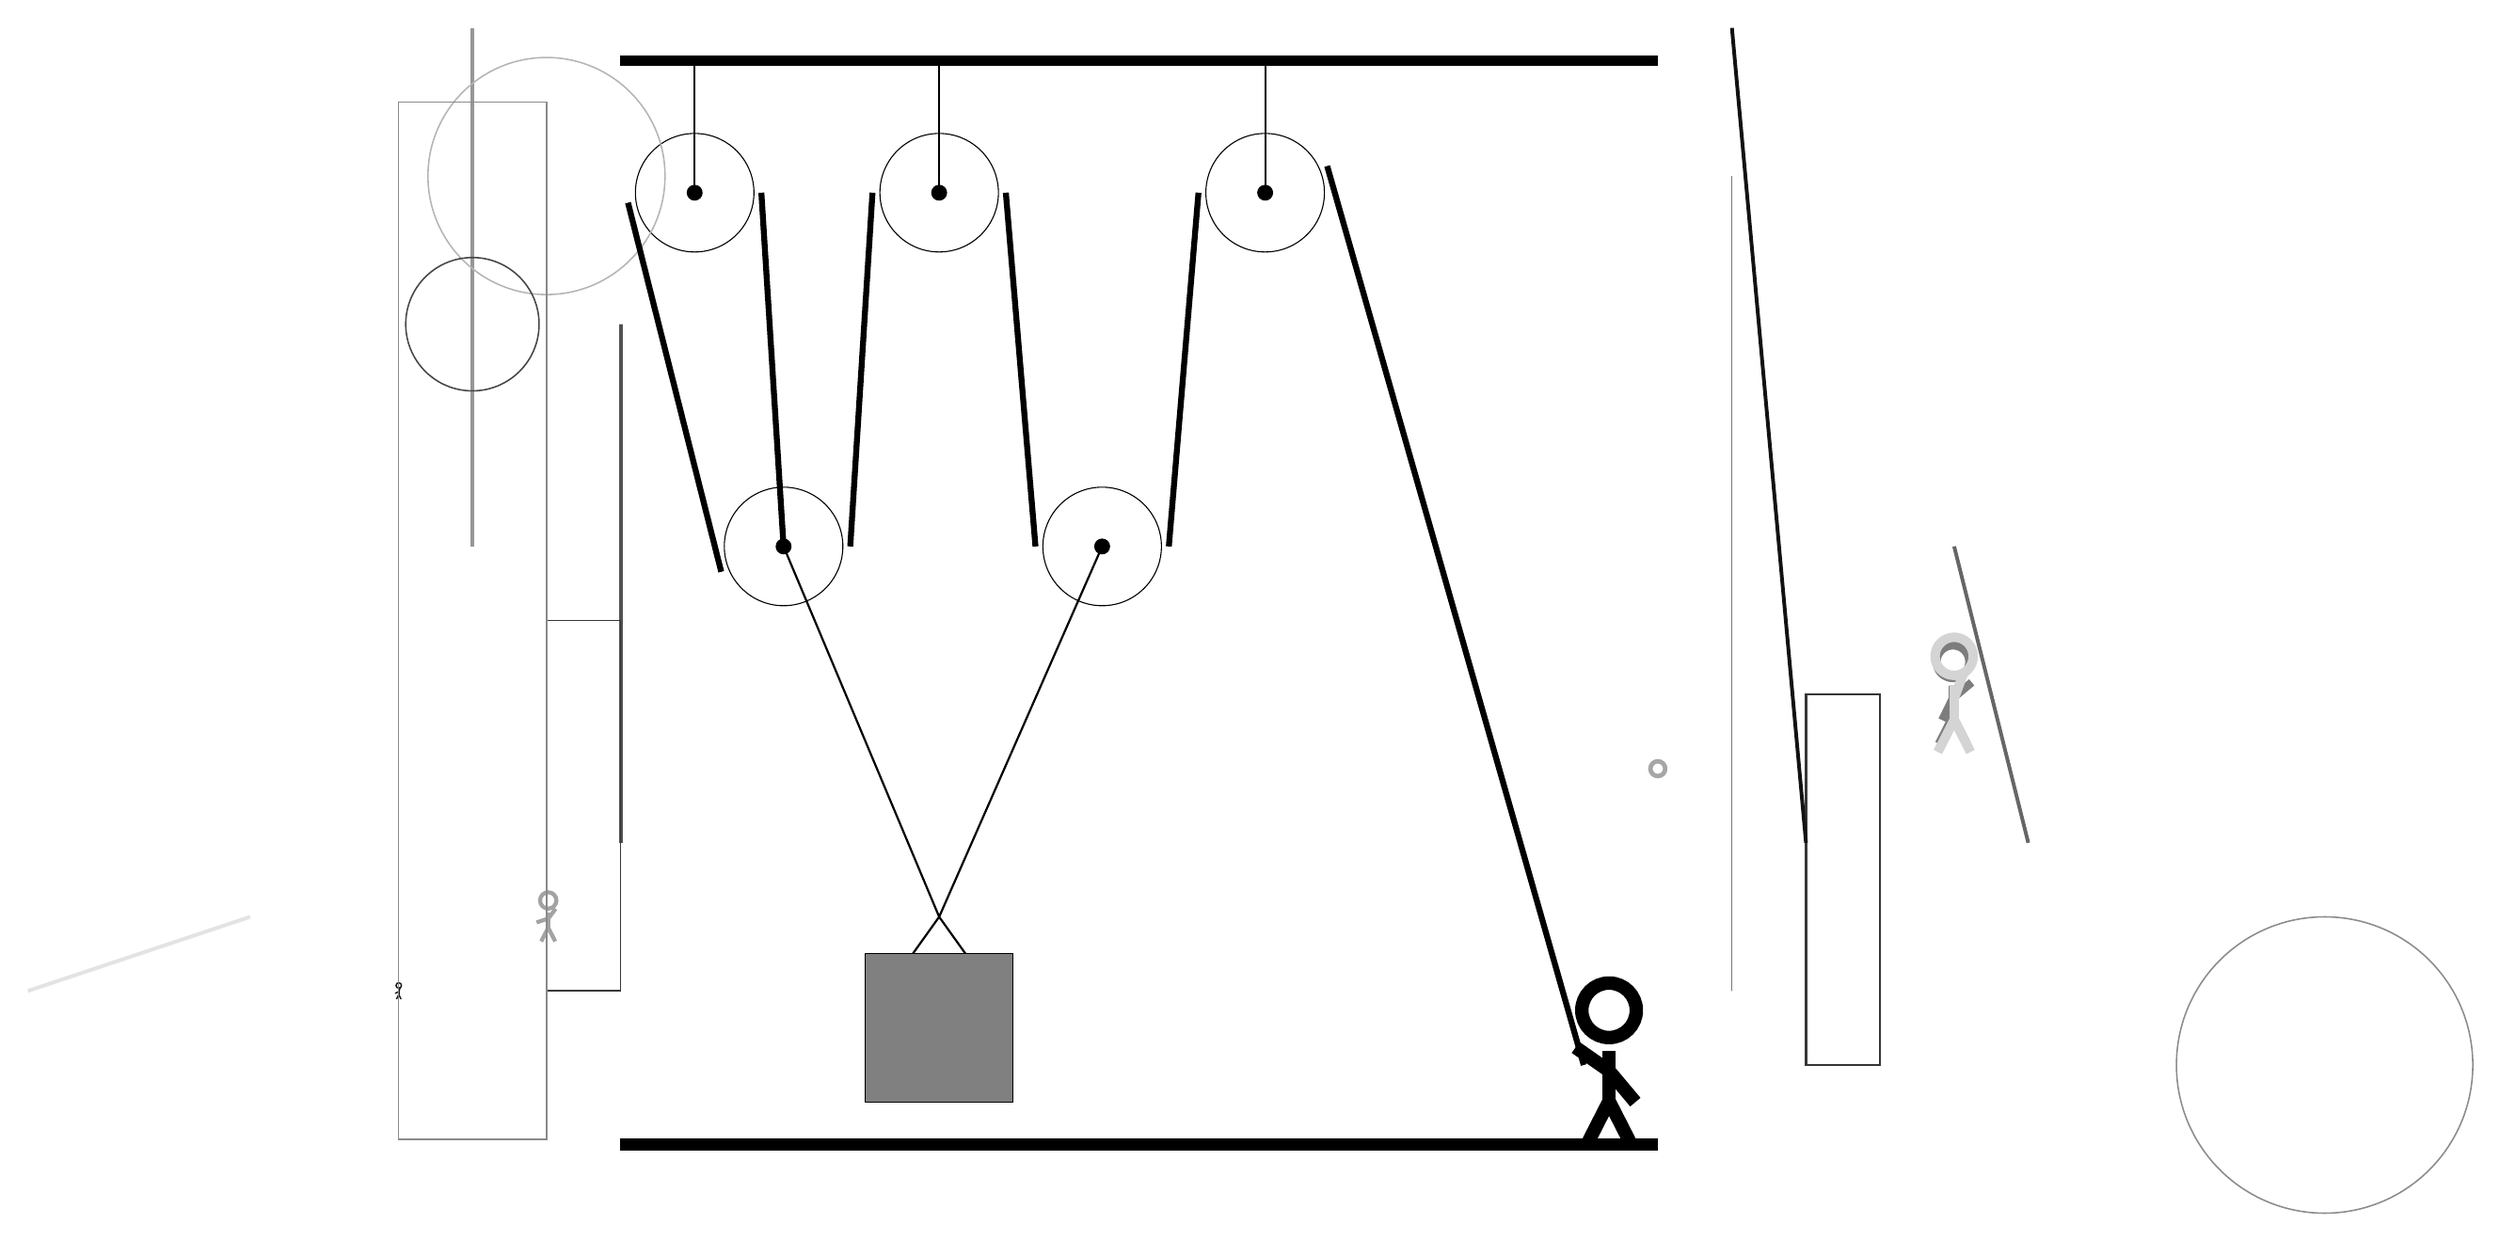
\begin{tikzpicture}
			%%%%% START %%%%%
			
			\draw[fill=black] (-2, 11.5) rectangle (12, 11.625);
			
			\draw (-1, 9.775) circle (0.8);
			\draw[fill=black] (-1, 9.775) circle (0.1);
			\draw[thick] (-1, 9.775) -- (-1, 11.5);
			
			\draw (2.3, 9.775) circle (0.8);
			\draw[fill=black] (2.3, 9.775) circle (0.1);
			\draw[thick] (2.3, 9.775) -- (2.3, 11.5);
			
			\draw (6.7, 9.775) circle (0.8);
			\draw[fill=black] (6.7, 9.775) circle (0.1);
			\draw[thick] (6.7, 9.775) -- (6.7, 11.5);
			
			\draw (0.2, 5) circle (0.8);
			\draw[fill=black] (0.2, 5) circle (0.1);
			
			\draw[line width=0.3mm, color=black!79] (14, -2) rectangle (15, 3);
			
			\draw[line width=0.5mm, color=black!60](17, 1) -- (16, 5);
			\draw[line width=0.5mm, color=black!68] (-2, 1) rectangle (-2, 8);
			\node[line width=0.4mm, color=black!51] at (16, 3) {\Strichmaxerl[6][64][40]};
			\node[line width=0.5mm, color=black!91] at (-5, -1) {\Strichmaxerl[1][28][69]};
			\draw[line width=0.2mm, color=black!78] (-2, -1) rectangle (-3, 4);
			\draw[line width=0.2mm, color=black!53] (13, -1) rectangle (13, 10);
			
			\node[line width=0.7mm, color=black!36] at (-3, 0) {\Strichmaxerl[3][18][53]};
			\draw[line width=0.5mm, color=black!41](-4, 5) -- (-4, 12);
			\draw [line width=0.2mm, color=black!29](-3, 10) circle (1.6);
			\draw [line width=0.2mm, color=black!72](-4, 8) circle (0.9);
			\draw[line width=0.5mm, color=black!93](14, 1) -- (13, 12);
			\draw[line width=0.5mm, color=black!11](-7, 0) -- (-10, -1);
			\draw [line width=0.6mm, color=black!35](12, 2) circle (0.1);
			\draw [line width=0.2mm, color=black!45](21, -2) circle (2.0);
			\draw[line width=0.2mm, color=black!46] (-3, 11) rectangle (-5, -3);
			\node[line width=0.3mm, color=black!17] at (16, 3) {\Strichmaxerl[7][90][70]};
			
			\draw (4.5, 5) circle (0.8);
			\draw[fill=black] (4.5, 5) circle (0.1);
			
			\draw[thick] (0.2, 5) -- (2.3, 0)  -- (4.5, 5);
			\draw[thick]  (1.8, -0.7) -- (2.3, 0) -- (2.8, -0.7);
			\draw[fill=black!50] (1.3, -0.5) rectangle (3.3, -2.5);
			
			\draw[line width=0.8mm] (0.2, 5) -- (-0.1, 9.775);
			\centerarc[line width=0.8mm](-1, 9.775)(0:200:0.9);
			\draw[line width=0.8mm] (-1.9, 9.64) -- (-0.6415, 4.658);
			\centerarc[line width=0.8mm](0.2, 5)(200:360:0.9);
			\draw[line width=0.8mm](1.1, 5) -- (1.4, 9.775);
			\centerarc[line width=0.8mm](2.3, 9.775)(0:180:0.9);
			\draw[line width=0.8mm] (3.2, 9.775) -- (3.6, 5);
			\centerarc[line width=0.8mm](4.5, 5)(180:360:0.9);
			\draw[line width=0.8mm] (5.4, 5) -- (5.8, 9.775);
			\centerarc[line width=0.8mm](6.7, 9.775)(20:180:0.9);
			\draw[line width=0.8mm](7.537, 10.135)  -- (11, -2);
			
			\node at (11.3, -2) {\Strichmaxerl[10][-35][-50]};
			
			\draw[fill=black] (-2, -3) rectangle (12, -3.15);
			
			%%%%% END %%%%%
		\end{tikzpicture}
	\end{figure}	
\end{document}